
An overview of the hardware and software resources that will be used in the project  is presented in this chapter. 

\subsubsection{Hardware Resources}

As \textbf{hardware resources}, the following components were identified:
\begin{itemize}
\item Zybo Board (Zynq-7000 ARM), which contains an ARM Cortex-A9 processor (for testing the hardware implementations).

\begin{figure}[!htb]
\centering
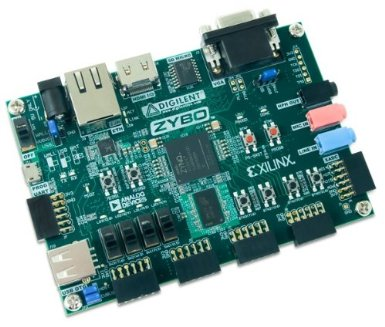
\includegraphics[scale=0.3]{images/Zybo.jpg}
\caption{Zybo Board (Zynq-7000 ARM).}
\label{fig:Zybo} 
\end{figure}

\item Microsemi's SmartFusion\textsuperscript{\textregistered} 2 Advanced Development Kit (ARMV7-M), which contains an ARM Cortex-M3 processor (platform that runs the DBT).
\end{itemize}

\begin{figure}[!htb]
\centering
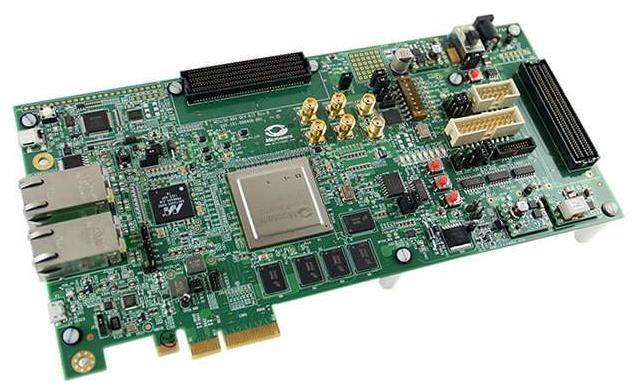
\includegraphics[scale=0.2]{images/SmartFusion2.jpg}
\caption{Microsemi's SmartFusion\textsuperscript{\textregistered} 2 Advanced Development Kit.}
\label{fig:SmartFusion} 
\end{figure}


\subsubsection{Software Resources}
As \textbf{software resources}, several tool will be used to achieve the purposes: 
\begin{itemize}
\item EL Framework.
\item DBT source files.
\end{itemize}


\begin{itemize}
\item Understand™ Static Code Analysis Tool.

\begin{figure}[!htb]
\centering

\includegraphics[scale=0.5]{images/Understand_logo}
\caption{Understand™}
\label{fig:Understand_logo} 
\end{figure}

\item IAR Embedded Workbench (IAR Systems) and C++ Language (for the modification of the DBT project).

\begin{figure}[!htb]
\centering

\includegraphics[scale=0.15]{images/IAR}
\caption{IAR Embedded Workbench }
\label{fig:IAR_logo} 
\end{figure}

\item Vivado Design Suite (Xilinx) and Verilog Language (for the development of the hardware implementation).

\begin{figure}[!htb]
\centering

\includegraphics[scale=0.2]{images/vivado_logo}
\caption{Vivado\textsuperscript{\textregistered} Design Suite}
\label{fig:Vivado_logo} 
\end{figure}

\item Eclipse IDE (for the development of the contents related to the \textit{EL} framework)

\begin{figure}[!htb]
\centering

\includegraphics[scale=0.2]{images/eclipse}
\caption{Eclipse\textsuperscript{\textregistered} IDE}
\label{fig:Eclipse_logo} 
\end{figure}

\end{itemize}

